\chapter[Validating lava flow simulators using a validation hierarchy and bayesian analysis]{Validating lava flow simulators using a validation hierarchy and bayesian analysis}\label{ch_molasses}

\renewcommand*{\FigPath}{figures/chapter-molasses}

\section*{Abstract}
	Modeling lava flows through cellular automata (CA) methods enables a computationally inexpensive means to quickly forecast lava flow paths and ultimate areal extents. A CA program has been created in the program language C that is modular, which enables a combination of governing CA rules to be evaluated against each other. My objective is to find a successful combination of automata behaviors that behaves like a bingham fluid and accurately forecasts lava inundation. To fulfill this objective, four validation levels have been devised, into which different tests can be applied to evaluate lava spreading algorithms against increasingly complex tests. These levels are 1) verification of the code by testing for conservation of mass; 2) testing for flow self-similarity given inconsequential variations in input parameters; 3) testing for replication of Bingham flow morphology on simple surfaces; and 4) testing for replication of real lava flow morphologies on pre-eruption elevation models. Two Bayesian posterior statistics, the Positive Predictive Value ($\text{Pr}(Lava|Sim)$) and the Negative Predictive Value ($\text{Pr}(\neg Lava|\neg Sim)$) are then used to further charactarize model performance against the 2012-3 Tolbachik lava flow. These metrics can provide insight into improving model performance and decision making in volcanic crises.

\section{Introduction}
	Lava flows as a gravity current on the surface of the Earth when liquid magma is effused at the surface with little or no explosivity. In the vacinity of active volcanoes, lava flows represent significant long term impact to infrastructure \citep{peterson2000lava}. In the past, lava flow hazard has been mitigated with the construction of physical diversions and at least once in 252 A.D. by the supernatural grace of St. Agatha of Sicily who died the year prior. Modern science suggests, however, that forecasting the flow path of lava from active volcanoes might be more useful than St. Agatha for communities impacted by effusive volcanism.

	Methods of forecasting lava flows range from simple predictions using empirical relationships between magma flux and flow length \citep{Glaze2003}, to 1-D numerical solutions such as FLOWGO \citep{harris2001flowgo}, to advanced computational fluid dynamics codes like lavaSIM \citep{hidaka2005vtfs}. All modern numerical flow models by nature trade precision in simulating physical processes with computer run-time, so that while FLOWGO is relatively fast it only predicts downslope flow length, while lavaSIM solves Navier-Stokes equations to produce a 3-D flow distribution at the expense of large computational requirements.
	
	Cellular Automata (CA) methods \citep{wolfram1984cellular} have been developed to simulate fluid flow, including lava spreading \citep{barca1994cellular}. In contrast to CFD codes, these do not generally attempt to compute Navier-Stokes equations but instead abstract many physical parameters, such as viscosity and temperature, into more or less empirical rules. The benefit of CA methods for simulating lava flows is most noticeable in the reduced computer time necessary for simulation compared to CFD methods.
	
	Multiple CA lava flow algorithms exist, such as SCIARA \citep{crisci2004simulation}, MAGFLOW \citep{del2008simulations}, ELFM \citep{damiani2006lava}, and LavaPL \citep{connor2012probabilistic}. These algorithms are variations on a theme, where the largest difference between each is how lava is distributed from one automaton to its neighbors. For instance, three versions of SCIARA allow for lava to spread in cardinal directions \citep{barca1994cellular}, in hexagonal directions \citep{crisci2008lava}, or in directions based on an inherent velocity calculated in an eulerian way for each automaton \citep{avolio2006sciara}. MAGFLOW and ELFM by contrast to the original SCIARA algorithm implements 8 directions of spreading. LavaPL and SCIARA both spread in four directions but the apportionment of lava from one automaton to neighbors is based on a different algorithm.

%%%%%%%%%%%%%
%Everything here down should likely be re-written

	While several lava flow simulators now exist, each have been made and tested with different lava flows or aspects of flows in mind. Because of this, selecting a specific algorithm to effectively model lava flow hazards can be a necessary, if unwanted challenge. To address this problem, we propose a hierarchical validation scheme to objectively test different flow spreading algorithms. Tests can be designed with different validation levels in mind, to compare lava flow simulations to increasingly complex models, from simply conserving mass to replicating the paths and ultimate areal extents of real lava flows. The tests described in this project can be applied to any flow algorithm that provides at least a list or map of inundated locations over various topographies.

	In this paper, multiple lava flow algorithms are tested using a new modular lava flow code, which I have named MOLASSES (standing for \textit{MOdular LAva Simulation Software in Earth Science}). This code, implemented in C, is a Cellular Automata code which tracks a population of equal-area spaced cells over a grid that is defined by a digital elevation model (DEM). These cells may or may not be inundated with lava and they are governed by universal rules. Because MOLASSES has been designed in a modular way, it is relatively quick to modify the flow algorithm. Using this code enables code output in a constant format, despite changing methods of lava distribution, which simplifies the comparison of methods.
	
	Several flow algorithms have been designed in MOLASSES. Each algorithm begins a lava flow simulation by delivering a user-defined amount of lava to one or more source cells (i.e. vents). Then another module distributes this lava across the elevation grid, before more lava is added to each source cell. When the total volume of lava defined by a user has been delivered to the flow, the simulation ends. The simulation algorithms vary by changing the rules of how lava is distributed across the map. For instance, some algorithms allow each grid cell in the lava flow to spread lava to neighbors in cardinal directions, while other algorithms spread lava from each cell in 8 directions. More detailed explanations of the MOLASSES code and different example implementations of the code are given in Appendix \ref{apdx_lava}.
	
	Eight MOLASSES flow algorithms are tested against a hierarchy of validation tests in Appendix \ref{apdx_lava}. %Validation tests are designed from Bayarri. While no algorithm is perfect, I will continue to use one of these because it performed best for Shuttle Radar Topo Mis topography data, which is what I'll use in the next section. It's called 8/N/S, which means that is shares in 8 dir, it does not have parent rules, and it shares lava prop to slope. This label is described in the appendix.
	
	%In the next subsection, I'll detail the location. In the following sections I will show how bayesian statistics can assess model validity, and estimate validity when parameter uncertainty is taken into account.
	
	
	%Several flow algorithms have been designed in MOLASSES, all of which pulse lava from a vent cell and distribute lava away from that cell across elevation models.
	%These algorithms have been tested using validation exercises
	%The outline and validation exercises are described in Appendix \ref{}
	%
	%In this paper I will use one of these algorithms which performs well under these exercises and flows in an 8/N/S way
	%I will use Tolbachik lava flow with SRTM topography
	%Bayesian section will do X
	
	%In Section \ref{sec:MOLASSES}, I will demonstrate how CA is applied to lava flows and detail how a CA simulation is carried out in the MOLASSES code. I will introduce a validation hierarchy in Section \ref{sec_validationb} that can be used to verify and validate different lava flow algorithms using increasingly complex model parameters. In Section \ref{sec:Bayesian}, I will expand on the final validation level (validation against real lava flows) with a Bayesian approach to improving model performance for the 2012-3 Tolbachik Lava Flow. The results from these Sections will be discussed in Section \ref{sec:discussion}.
	
	\subsection{Case study area: 2012-3 Tolbachik Lava Flow}\label{sec_tolb_back}
	%In the third validation level (Section \ref{sec_tolb_bench}), the recent lava flows at Tolbachik will be used as an example validation test to evaluate flow algorithms against a real lava flow. These flows will then be used in Section \ref{sec:Bayesian} as examples of how a Bayesian approach to evaluating model performance can improve model performance. 
	
\begin{figure}[!h]
	\centering
	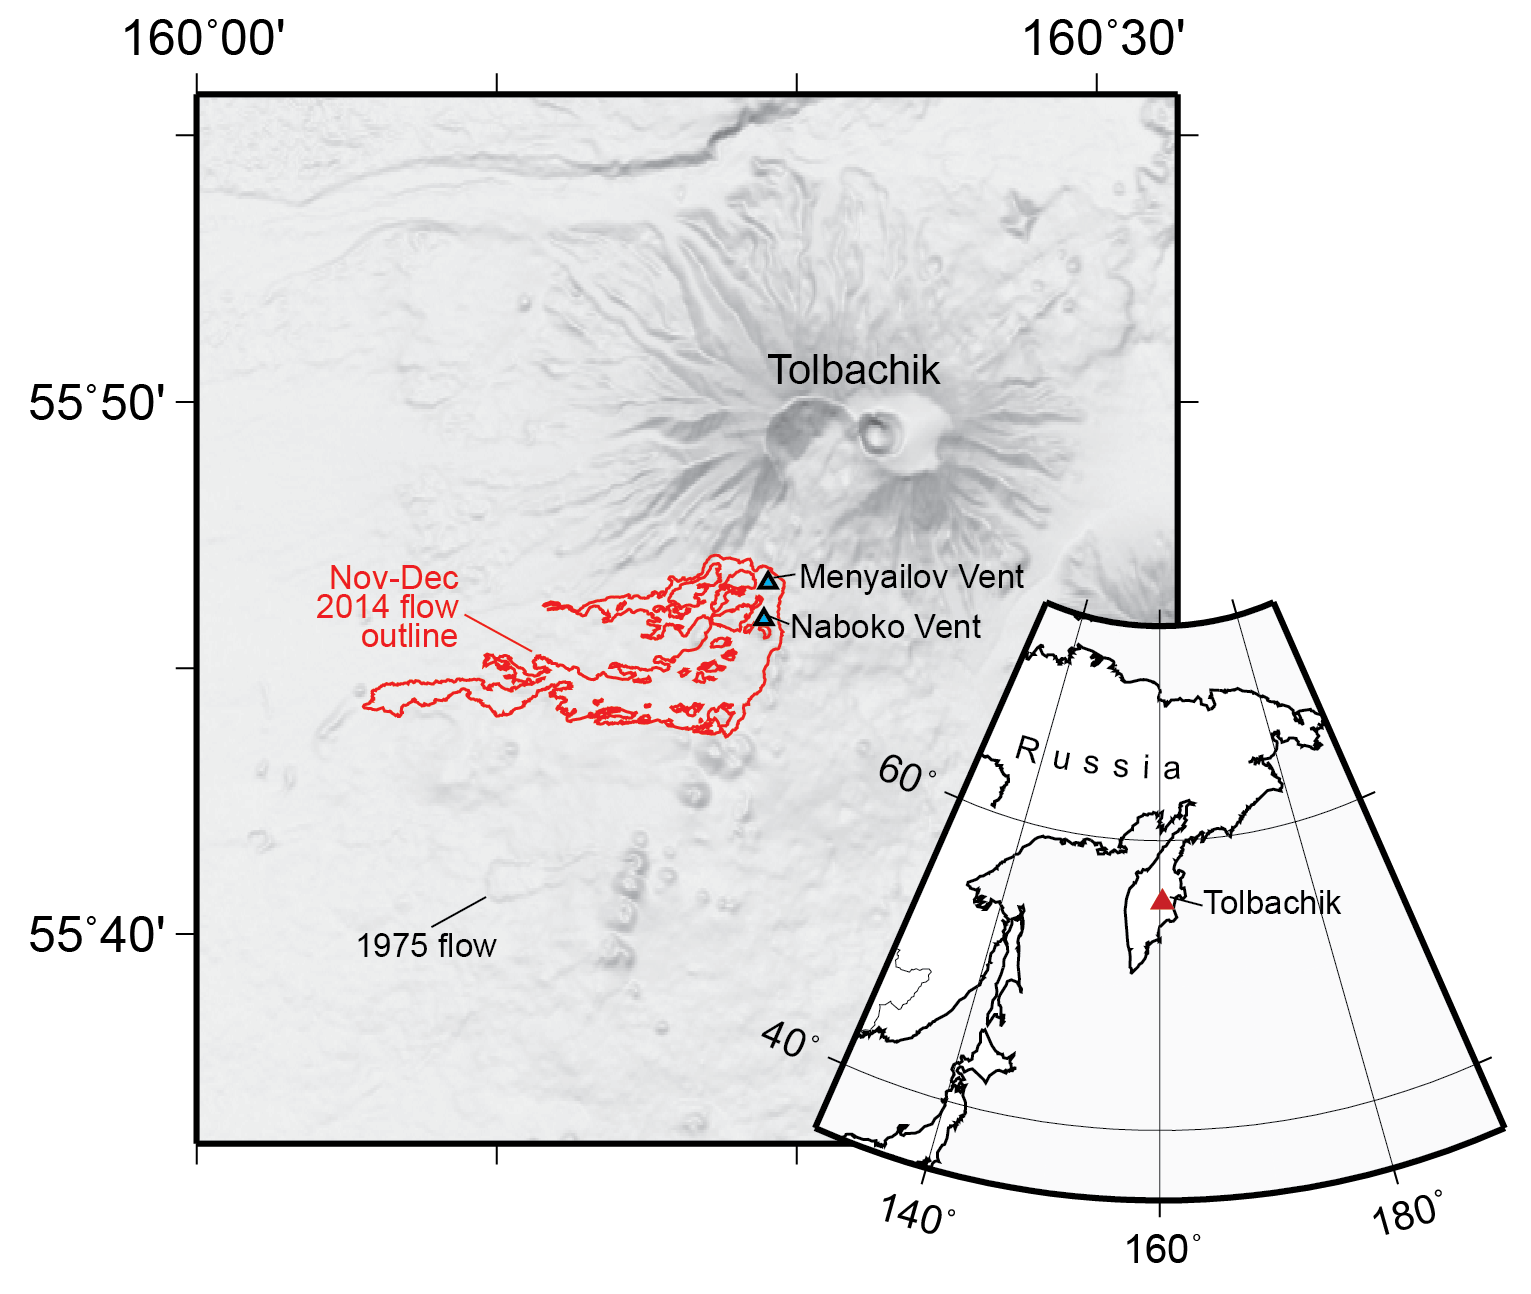
\includegraphics[width=0.7\linewidth]{\FigPath/locator_complete_300dpi}
	\caption[The Tolbachik region of Kamchackta, Russia]{The Tolbachik region of Kamchackta, Russia. The two main vents are shown as triangles and the outline of western lava flows, emplaced in 2014, is drawn in red.}
	\label{fig_locator}
\end{figure}
	
The Tolbachik lava flow began in November 2012, originally being sourced from a long fissure vent south of Tolbachik Dol. Initial magma flux was estimated to be 440~m$^3$~s$^{-1}$ \citep{belousov2015overview}. The fissure vent ultimately coalesced into two main vents, seen in TanDEM-X interferometric synthetic aperture radar (InSAR) data \citep{kubanek2015lava}, and the flux dropped significantly to between 100 and 200~m$^3$~s$^{-1}$. Early stages of the flow carried lava west to a maximum runout of 14.5~km and later stages beginning in January or February, carried lava east. The total emplacement volume is $\sim$0.53$\pm$0.07~km$^3$ with 0.38~km$^3$ of that being to the west. TanDEM-X InSAR data has been used to show that the modal thickness of the flow is 7.8~m, and that the overall thickness distribution is log-normal \citep{kubanek2015lava}. After the flow ceased, the total emplacement area was mapped using orthophotos and TanDEM-X data where clouds were present in the images by \citet{kubanek2015lava}.

Figure \ref{fig_locator} shows the outline of the early lava flows, which traveled from two vents along a fissure to the west. This areal extent will be used to validate lava flow simulators. The flow volume is taken to be the total emplacement area within this outline, 26~km$^2$, multiplied by the observed modal thickness of the flow, 7.8~m. The total flow volume used the input parameter in the flow simulations will be 0.22~km$^3$. The remainder of the total emplacement volume to the west of the vents, 0.16~km$^3$ is interpretted to be material that built near-vent edifices (e.g. cones) \citep{kubanek2015lava}. The volume interpretted to be emminated from the northern vent is $4.63\times 10^7$~km$^3$, while the southern vent volume is $1.74\times 10^8$~km$^3$. This estimate was made by splitting the flow between areas north of the Menyailov (northern) vent and south of it, assuming that flows from the Menyailov vents traveled north.
	





%%%%%%%%%%%%%%%%%%%%%%%%%%%%%%%%%%%%%%%%%%%%%%%%
%%%%%%%%%%%%%%%%%%%%%%%%%%%%%%%%%%%%%%%%
%%%%%%%%%%%%%%%%%%%%%%%%%%%%%%%%%
%%%%%%%%%%%%%%%%%%%%%%%%%%
%%%%%%%%%%%%%%%%%%%
%%%%%%%%%%%%%%%%%%%%%%%%%%%%%%%%%%%%%%%%%%%%%%%%
%HERE IS WHERE THE BIG SECTIONS WERE REMOVED
%%%%%%%%%%%%%%%%%%%%%%%%%%%%%%%%%%%%%%%%%%%%%%%%
%%%%%%%%%%%%%%%%%%%%%%%%%%%%%%%%%%%%%%%%%%%%%%%%
%%%%%%%%%%%%%%%%%%%%%%%%%%%%%%%%%%%%%%%%%%%%%%%%
%SECTION: CELLULAR AUTOMATA EXPLANATION
%SECTION: VALIDATION OF CODE
%%%%%%%%%%%%%%%%%%%%%%%%%%%%%%%%%%%%%%%%%%%%%%%%
%%%%%%%%%%%%%%%%%%%%%%%%%%%%%%%%%%%%%%%%
%%%%%%%%%%%%%%%%%%%%%%%%%%%%%%%%%
%%%%%%%%%%%%%%%%%%%%%%%%%%
%%%%%%%%%%%%%%%%%%%






%%%%%%%%%%%%%%%%%%%%%%%%%%%%%%%%%%%%%%%%%%%%%%%%
%BAYESIAN APPROACH
%%%%%%%%%%%%%%%%%%%%%%%%%%%%%%%%%%%%%%%%%%%%%%%%
%%%%%%%%%%%%%%%%%%%%%%%%%%%%%%%%%%%%%%%%%%%%%%%%
%%%%%%%%%%%%%%%%%%%%%%%%%%%%%%%%%%%%%%%%%%%%%%%%
\section{Bayesian applications for lava flow models}\label{sec:Bayesian}
	The final step \citet{bayarri2007framework} give for validating computer models is ``feeding [observations and results] back to revise the model.''
	
	The use of computer models to forecast hazards is a fundamentally Bayesian strategy: there is an initial concern due to hazards and computer models help us inform, constrain, and update this concern. Using Bayesian statistics can therefore be an improvement in testing lava flow models, over the two commonly used fitness tests, model sensitivity and the Jaccard index, because of their more direct application to informing perceived risk. 
	
	Three tools will be used in this section: the Positive Predictive Value, the Negative Predictive Value, and a Bayes factor. Bayes theorem connects a phenomenon $A$ to observations $B$ through the function
	\begin{equation}
		\text{Pr}(A|B)=\frac{\text{Pr}(B|A)\text{Pr}(A)}{\text{Pr}(B)}\label{eq_bayes}
	\end{equation}
	where $\text{Pr}(A)$ is the general probability of $A$ occuring, $\text{Pr}(B)$ is the probability of $B$ being observed, and $\text{Pr}(B|A)$ is the conditional probability of $B$ given the occurence of $A$. $\text{Pr}(B|A)$ is also known as model sensitivity, which is a common fitness statistic and was discussed in Section \ref{sec_tolb_bench}
	
	The left side of Equation \ref{eq_bayes}, $\text{Pr}(A|B)$, is the Posterior probability of $A$ and can be stated as ``the probability that lava will inundate a location if the model forecasted inundation at that location,'' or the Positive Predictive Value (PPV) of the model. A second posterior is the Negative Predictive Value (NPV) and is $\text{Pr}(\neg A|\neg B)$, the obverse of $\text{Pr}(A|B)$. This negative predictive value relates not being inundated by lava at a given location to a safe outcome forecasted by a simulation and can be calculated by modifying Equation \ref{eq_bayes} and substituting $A$ for $Lava$ (the lava flow) and $B$ for $Sim$ (the simulation), resulting in the formula
	\begin{equation}
		\text{Pr}(\neg Lava|\neg Sim)=\frac{\text{Pr}(\neg Sim|\neg Lava)\text{Pr}(\neg Lava)}{\text{Pr}(\neg Sim)}
	\end{equation}
	where the $\neg$ symbol indicates the event or observation not happening, and $\text{Pr}(\neg Sim|\neg Lava)$ is model specificity.
	
	The negative predictive value is important in hazard forecasting as it is in some sense a probability of safety. The more common positive predictive value $\text{Pr}(A|B)$ (or $\text{Pr}(Lava|Sim)$) does not contain information about areas that the simulation does not inundate, as it is essentially the True Positive area divided by the area of simulated inundation (defined later in Equation \ref{eq_simplepost}). While the PPV can support the hypothesis that lava will hit a location given a simulated hit, it cannot estimate one's relative risk if the simulation forecasts a safe outcome. The NPV, $\text{Pr}(\neg Lava|\neg Sim)$, does just this, and informs a user whether to rely on a safe outcome from a simulation. If, for example, the PPV $\text{Pr}(Lava|Sim)$ is high while the NPV $\text{Pr}(\neg Lava|\neg Sim)$ is low for a given lava flow simulator, areas that are evacuated due to the simulation outcome will be evacuated for good reason, but many areas will likely be inundated that were not evacuated due to the simulation outcome. It is important to estimate and ultimately try to improve both predictive values, because it is important to understand both how well a simulation matches areas inundated by lava and how well it matches areas not inundated by lava.
	
	Bayes factors provide a tool to test the relative likelihood of a hypothesis against another. \citet{aspinall2003evidence} introduced this tool to volcano hazard forecasting by testing whether the onset of particular seismic events before the 1993 Galeras catastrophe was a significant indicator of the eruption or not. A Bayes Factor (BF) relating two hypotheses is given by \citet{jeffreys1998theory} as
	\begin{equation}
		\text{BF} = \frac{\text{Pr}(\text{Evidence}|\text{Hypothesis~1})}{\text{Pr}(\text{Evidence}|\text{Hypothesis~2})}
		\label{eq_BF}
	\end{equation}
	In the example of Galeras, the Evidence in Equation \ref{eq_BF} are new seismic events, Hypothesis 1 is ``imminent explosion,'' and Hypothesis 2 is its complement ``not imminent explosion'' \citep{aspinall2003evidence}. Below, I will apply this with the Evidence being the probability of simulated inundation and the Hypotheses ``lava inundation'' and ``not lava inundation.'' Essentially, the Bayes Factor approach identifies whether an area, given evidence provided by flow simulations, is better described as inundated by lava or not inundated by lava. \citet{jeffreys1998theory} provided a log-scale interpretation to the value of BF in Equation \ref{eq_BF}, given in the Table \ref{tab_BFinterps}.
	
	\begin{table}[h]
		\centering
		\caption{Bayes Factor Interpretations (modified from \citet{aspinall2003evidence})}
		\begin{tabular}{l l}
			\toprule
			BF Value & Description\\
			\midrule
			$BF>10^2$ & Evidence for Hypothesis 1 is Decisive.\\
			$10^{1.5}<BF<10^2$ & Evidence for Hypothesis 1 is Very Strong.\\
			$10^{1}<BF<10^{1.5}$ & Evidence for Hypothesis 1 is Strong.\\
			$10^{0.5}<BF<10^{1}$ & Evidence for Hypothesis 1 is Substantial.\\
			$10^{0}<BF<10^{0.5}$ & Evidence for Hypothesis 1 is just worth a mention.\\\\
			$10^{-0.5}<BF<10^{0}$ & Evidence for Hypothesis 2 is just worth a mention.\\
			$10^{-1}<BF<10^{-0.5}$ & Evidence for Hypothesis 2 is Substantial.\\
			$10^{-1.5}<BF<10^{-1}$ & Evidence for Hypothesis 2 is Strong.\\
			$10^{-2}<BF<10^{-1.5}$ & Evidence for Hypothesis 2 is Very Strong.\\
			$BF<10^{-2}$ & Evidence for Hypothesis 2 is Decisive.\\
			\bottomrule
		\end{tabular}
		\label{tab_BFinterps}
	\end{table}
	
		\paragraph{Calculating predictive values} In the same manner as the final validation level, the statistics discussed above will be calculated based on the areal extent of flows and simulations. The probability of the lava flow inundating an area $N$ can be given as
		\begin{equation}
			\text{Pr}(A)=\frac{|Lava|}{|N|}\label{eq_PA}
		\end{equation}
		where $|Lava|$ is the areal size of the flow (i.e. literally the number of DEM grid cells the lava inundates) and $|N|$ is the size of the area of interest, or the potential hazard area. The probability of the simulation is similarly found to be
		\begin{equation}
			\text{Pr}(Sim)=\frac{|Sim|}{|N|}.\label{eq_PB}
		\end{equation}
		By substituting these definitions and model sensitivity (Equation \ref{eq_sensitivity}, $|Lava \cap Sim|/|Lava|$) in Equation \ref{eq_bayes}, the posterior probability of lava flow inundation (i.e. the PPV), given a simulation that forecasts inundation can be recast as
		\begin{align}
		\text{Pr}(Lava|Sim)&=\frac{\frac{|Lava\cap Sim|}{|Lava|}\frac{|Lava|}{|N|}}{\frac{|Sim|}{|N|}}~\text{,~or~simplified,}\label{eq_unsimplepost}\\
		&=\frac{|Lava\cap Sim|}{|Sim|}.\label{eq_simplepost}
		\end{align}
		where $|Lava\cap Sim|$ is the size of the intersection of the lava flow and simulated flow (again, the number of DEM grid cells that are True Positives). Note that PPV is independent of the potential hazard area.
		
		the NPV can be stated in terms of the sizes of the lava flow and simulated flow as well.
		\begin{equation}
			\text{Pr}(\neg Lava|\neg Sim)=\frac{|\neg Lava\cap \neg Sim|}{|\neg Sim|}\label{eq_simplenegpost}
		\end{equation}
		In this equation the numerator is the total area of True Negatives, where neither real flows or simulated flows reached. The denominator is the area not hit by the simulated flows, or the True and False Negatives. Calculating the size or number of grid cells of $\neg Lava$ or $\neg Sim$ is fundamentally dependent on the potential hazard area, as $|\neg Lava|$ is defined as
		\begin{equation}
			|\neg Lava| = |N| - |Lava|.
		\end{equation}
		Because of this, we must define the size of the potential hazard area $N$ ($|N|$).	
	
	\paragraph{Potential hazard area} There are multiple strategies to estimating an \textit{a priori} hazard area. \citet{kauahikaua1995applications} for instance identified catchments or ``lava sheds'' in which a volcanic vent was erupting, and identified these lava sheds as the hazard area. \citet{kilburn2000lava} provided a theoretical maximum distance that a lava flow can travel given the mass flux of magma erupting at the vent location. A combination of these two would provide an objective hazard area defined as the area within the ``Kilburn distance'' that is topographically below the volcanic vent. The theoretical maximum distance, or hazard radius, given by \citet{kilburn2000lava} is
		\begin{equation}
		R_{max}=\sqrt{\frac{3\epsilon SQ}{\rho g\kappa}}
		\label{eq_kilburn}
		\end{equation}
	where $\epsilon$ is an empirical value related to the amount of extension of lava crust allowed before it fails (10$^{-3}$), $S$ is the tensile strength of this crust (10$^7$~Pa), $\rho$ is the lava crust density (2200~kg~m$^{-3}$), $g$ is gravitational acceleration, $\kappa$ is the bulk thermal diffusivity ($4\times 10^{-7}$~m$^{2}$~s$^{-1}$) and $Q$ is the mean volumetric flow rate from the vent. From this, the hazard radius for the Tolbachik 2012-3 flow is calculated to be 39~km, given a magma flux of 440~m$^3$~s from the vent as was estimated early in the eruption \citep{belousov2015overview}. The total area within this radius that is also below the vent-plus-modal-flow-thickness elevation is 1,415~km$^2$. Note that the mapped flow area of 26~km$^2$ only covers 1.9\% of this defined hazard area (i.e. $\text{Pr}(Lava) = 0.019$).
	
		\begin{figure}
			\centering
			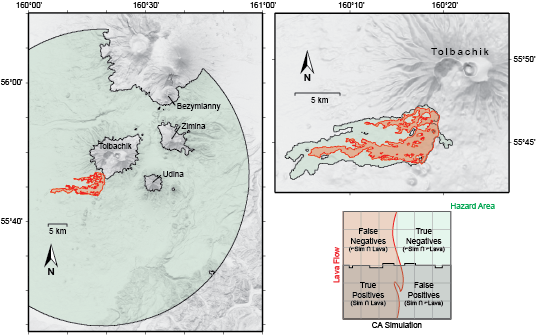
\includegraphics[width=0.7\linewidth]{\FigPath/hazard_areas_72dpi}
			\caption[Potential hazard areas of the 2012-3 Tolbachik Flows]{Potential hazard areas of the 2012-3 Tolbachik Flows. Hazard areas, shaded light green, are defined by a maximum flow radius (left, Equation \ref{eq_kilburn}) and the total areal coverage of 100,000 random flow simulations (top-right, Section \ref{sec_MC}). The mapped lava flow is red. The chart to the bottom right shows the 2x2 grid illustrated in Figure \ref{fig_2x2}.}
			\label{fig_hazardarea}
		\end{figure}
	
	A second strategy would be to run many lava flow models from the known vent location(s) while varying input parameters. This would give a range of flows and the true flow might be completely contained within the region given by this range of simulations. Below, a Monte Carlo (MC) method will be used to simulate a large range of flows. If we define a potential hazard area as any location inundated by at least one simulated flow in this MC approach, the hazard area would be 72~km$^2$. As the mapped flow area from the Tolbachik eruption is 39\% of this area, it would be more practical to use this as the \textit{a priori} hazard area because it more reasonably reflects the potential inundation area. Both the Kilburn-Kauahikaua method and this MC method are illustrated in Figure \ref{fig_hazardarea}.				
	
	\paragraph{Review of validation level 3} Instead of using model sensitivity and the Jaccard index as fitness values for the various lava flow models, now the two predictive values will be used. The potential hazard area is defined as the distribution of MC simulations (72~km$^2$). To give an example calculation, $\text{Pr}(Lava|Sim)$ is found with Equation \ref{eq_simplepost} by dividing true positives (green boxes in \ref{fig:tolbachik}) by the simulation area (green and red boxes). The NPV, $\text{Pr}(\neg Lava|\neg Sim)$, is found by diving true negatives (top right of Figure \ref{fig_2x2}), by the area not simulated (top half of Figure \ref{fig_2x2}). Table \ref{tab_fitmetriccompare} lists the fitness values from Table \ref{tab_tolbflowresults} as well as the two predictive values for eight flow simulation algorithms.
	
		\begin{table}[h]
		\centering
		\caption{Traditional Fit Metrics and Bayesian Posterior Functions}\\
		\begin{tabular}{l c c c c}
			\toprule
			Transition&\multicolumn{4}{c}{\textbf{Results of simulations over SRTM DEM}}\\
			Function& Jaccard & Sensitivity & Pos. Pred. Value & Neg. Pred. Value\\
			\midrule
			4/P/S & 56.7\%& 76.4\%& 70.4\%& 84.5\% \\
			8/P/S & 61.1  & 80.8  & 73.2  & 87.3   \\
			4/N/S & 57.2  & 77.5  & 70.3  & 85.1   \\
			8/N/S & 63.1  & 82.8  & 74.4  & 88.5   \\
			4/P/E & 51.2  & 71.5  & 66.0  & 81.4   \\
			8/P/E & 58.8  & 78.2  & 72.0  & 85.7   \\
			4/N/E & 54.5  & 74.5  & 68.7  & 83.3   \\
			8/N/E & 59.6  & 78.8  & 72.8  & 86.2   \\
			
			\bottomrule
		\end{tabular}
		\label{tab_fitmetriccompare}
	\end{table}
	
	For the rest of this section, the 8/N/S (the 8-connected, no parent-child relationships, with slope-proportional spreading) algorithm will be used. This is preferred because it out-performed other algorithms over the SRTM DEM. By applying this model to the Tolbachik lava flows, Bayesian methods will be used to improve the ``Pulse Volume'' parameter and will later be used to constrain model uncertainty at Tolbachik.
	
	\subsection{Improving model performance on one model parameter}\label{sec_bayespulse}
	In the Tolbachik validation tests given as examples of comparing simulation algorithms against real lava flows (Section \ref {sec_tolb_bench}), all but one algorithm performed worse on the TanDEM-X derived elevation model. This was in part due to large run-out distances in the simulations (e.g. bottom right of Figure \ref{fig:tolbachik}), which considerably increased simulation false positives. The large run-out distances might be due to the pulse volume, the volume of lava given to source cells at each code loop in MOLASSES, being poorly chosen. Here, the Bayesian statistics defined above will be used to compare different pulse volumes and identify an optimal pulse volume. 
		
		An optimal pulse volume will ideally produce a flow simulation with the highest PPV and NPV. Pulse volumes with high associated PPVs will produce simulations where areas simulated as inundated by lava will have a high likelihood of actually being inundated by lava. Pulse volumes with high associated NPVs will produce simulations where areas simulated to not be inundated will hava a high likelihood of actually not being inundated.
		
		\subsubsection{Model execution} 
		To populate $Sim$, I have run the MOLASSES lava flow code using TanDEM-X derived parameters listed in Table \ref{tab_parameters_pulsebayes}. All variables are fixed except the pulse volume parameter, which is the amount of lava delivered to source cells in the Cellular Automata grid of MOLASSES. The lowest pulse volume, 1755 m$^3$ per pulse, is approximately the product of the TanDEM-X DEM grid cell size (225~m$^2$) and the residual flow thickness (7.8~m). The other 15 pulse volumes are multiples of this volume (i.e. they are 1.5 to 8.5$\times$ 1775 m$^3$).
		
		\begin{table}[h!]
		\centering
			\caption{MOLASSES Flow Parameters}
			\begin{tabular}{l l}
				\toprule
				Elevation Model & 15-m bistatic TanDEM-X, 11 Nov 2015\\
				Modal Thickness & 7.8~m\\
				Pulse Volumes & 16 equally separated volumes, [1755,14917] m$^3$\\
				\midrule
				Vent$_N$ Easting & 582800~m (UTM Zone 57)\\
				Vent$_N$ Northing & 6182100~m\\
				Vent$_N$ Total Volume & 4.63$\cdot10^7$~m$^3$\\
				\midrule
				Vent$_S$ Easting & 582475~m\\
				Vent$_S$ Northing & 6180700~m\\
				Vent$_S$ Total Volume & 1.737$\cdot10^8$~m$^3$\\
				\bottomrule
			\end{tabular}
			\label{tab_parameters_pulsebayes}
		\end{table}
		

		Model output is compared to a list of x,y locations in the Tolbachik area that have been inundated or not. This location list is stored in a raster with the same projection and extent as the elevation model used in MOLASSES. ASCII locations output by MOLASSES are also listed in the same projection within the same extent as the elevation model. This enables direct comparison between the Model information (i.e. $Sim$) and the mapped lava flow (i.e. $Lava$). True Positives, False Positives, and False Negatives are reported as cell counts (number of grid locations where $Lava$ and $Sim$ agree or not). Three examples of these simulations are mapped in Figure \ref{fig:pulse_map}.

		\begin{figure}
		\centering
		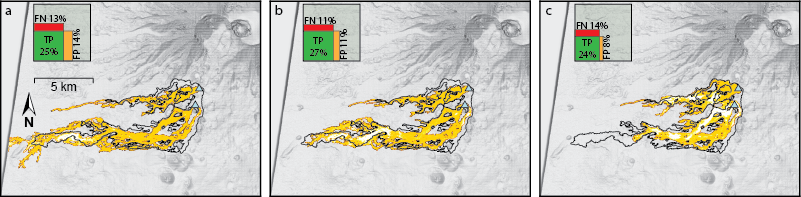
\includegraphics[width=\linewidth]{\FigPath/pulse_examples_72dpi}
		\caption[MOLASSES Simulations with different pulse volume parameter values of the 2012-3 Tolbachik Lava Flows]{MOLASSES Simulations with different pulse volume parameter values of the 2012-3 Tolbachik Lava Flows. Vents are shown as blue triangles and the mapped flow is outlined in black. a) Pulse Volume = 1755 m$^3$, the simulation far exceeds the true runout distance; b) Pulse Volume = 4387 m$^3$, this simulation performs best under the NPV $\text{Pr}(\neg Lava|\neg Sim)$ test; c) Pulse Volume = 14040 m$^3$, this simulation performs best under the PPV $\text{Pr}(Lava|Sim)$ test, but does not have a runout length similar to the mapped flow.}
		\label{fig:pulse_map}
		\end{figure}

		\subsubsection{Results}
		
		Three example simulations are shown in Figure \ref{fig:pulse_map} using simulation parameters from Table \ref{tab_parameters_pulsebayes} and different pulse volume values. With increased pulse volume, simulated run-out distance is shorter. This is because the MOLASSES code ends once all volume is delivered to the vents and the DISTRIBUTE module has run once more. In other words, if the pulse volume is doubled, the number of times the PULSE and DISTRIBUTE modules will be run will be halved, as the total volume will be delivered to the vents in half the code loops (see Figure \ref{fig_flowchart}). By running DISTRIBUTE fewer times, cells have fewer opportunities to advect lava downslope.

		The positive predictive value is the fundamental tool of Bayesian statistics, and quantifying it enables an update of belief in risk of lava inundation. A perfect PPV would mean that if the model simulates lava inundating a location, lava will certainly inundate that location. PPV is calculated for simulated lava flows of different Pulse Volumes and is graphed in Figure \ref{fig_lavaGsim}. From this, it can be seen that the highest pulse volumes, which coincidentally form the shortest flow simulations, perform best with this test, with the best fit having a pulse volume of 14040~m$^3$ per algorithm loop (Figure \ref{fig:pulse_map},c). A local maximum does exist in the low pulse volumes at 4387~m$^3$ per loop.


		\begin{figure}[h!]
			\centering
			\begin{gnuplot}[terminal=latex, terminaloptions=rotate]
				unset key
				set size 0.7,0.7
				set format xy "$%g$"
				set xlabel "Pulse Volume (m$^3$)" rotate by 90
				set ylabel "Pr$(Lava|Sim)$"
				set ytics 0.05
				set xtics 4000
				plot "data/results_bayes.dat" using 1:2 with linespoints lt 4 pt 7
			\end{gnuplot}
			\caption{PPV, $\text{Pr}(Lava|Sim)$, for MOLASSES flows with differing Pulse Volumes.}
			\label{fig_lavaGsim}
		\end{figure}
		
		The negative predictive value $\text{Pr}(\neg Lava|\neg Sim)$, is the percentage of non-inundated area in the simulation that is also not inundated in real life. A perfect NPV would indicate that, if a model does not simulate a hit for a location, lava will certainly not inundate that location. The NPV of simulations with different pulse values are shown in Figure \ref{fig_neglavaGsim}. Unlike the previous predictive value analyzed, the best performing flows, according to NPV, have smaller pulse volumes and the best performing volume is 4387~m$^3$ per model pulse loop (Figure \ref{fig:pulse_map},b).

		\begin{figure}[h!]
			\centering
			\begin{gnuplot}[terminal=latex, terminaloptions=rotate]
				unset key
				set size 0.7,0.7
				set format xy "$%g$"
				set xlabel "Pulse Volume (m$^3$)" rotate by 90
				set ylabel "Pr(not $Lava|$not $Sim)$"
				set ytics 0.01
				set xtics 4000
				plot "data/results_bayes.dat" using 1:3 with linespoints lt 4 pt 7
			\end{gnuplot}
			\caption{NPV, $\text{Pr}(\neg Lava|\neg Sim)$, for MOLASSES flows with differing Pulse Volumes.}
			\label{fig_neglavaGsim}
		\end{figure}
	
	\subsection{Incorporating model uncertainty with a Monte Carlo method}\label{sec_MC}
		Model uncertainty is a result of input parameter uncertainty, such as uncertainty in the underlying DEM. This can be distinguished from model error, which might be defined as the difference between the true lava flow and a simulation carried out with perfect input parameters, and is created by the inherent deviations between a computer model and real life processes. Because there is parameter uncertainty, it is essential to quantify the range of model solutions given the likely range of each parameter.
		
		In this example, elevation uncertainty will be examined. Elevation uncertainty is an element in the MOLASSES module \textbf{INITFLOW}, where each grid cell elevation can be defined randomly before the lava flow simulation begins. The user can add an elevation uncertainty, in meters, to the configuration file. If this value is provided, each grid cell will receive a new elevation value randomly selected from a normal distribution whose mean is the DEM elevation and the standard deviation is the uncertainty value.
		
		\begin{table}[h!]
		\centering
			\caption{Monte Carlo MOLASSES Flow Parameters}
			\begin{tabular}{l l}
				\toprule
				Elevation Model & 75-m SRTM\\
				Elevation Uncertainty, $1\sigma$ & 3~m\\
				Residual Thickness & 7.8~m\\
				Pulse Volume & 44200 m$^3$\\
				\midrule
				Vent$_N$ Easting & 582800~m (UTM Zone 57)\\
				Vent$_N$ Northing & 6182100~m\\
				Vent$_N$ Total Volume & 4.63$\cdot10^7$~m$^3$\\
				\midrule
				Vent$_S$ Easting & 582475~m\\
				Vent$_S$ Northing & 6180700~m\\
				Vent$_S$ Total Volume & 1.737$\cdot10^8$~m$^3$\\
				\bottomrule
			\end{tabular}
			\label{tab_parameters_MC}
		\end{table}
		
		%Map of the MC flows
		\begin{figure}
			\centering
			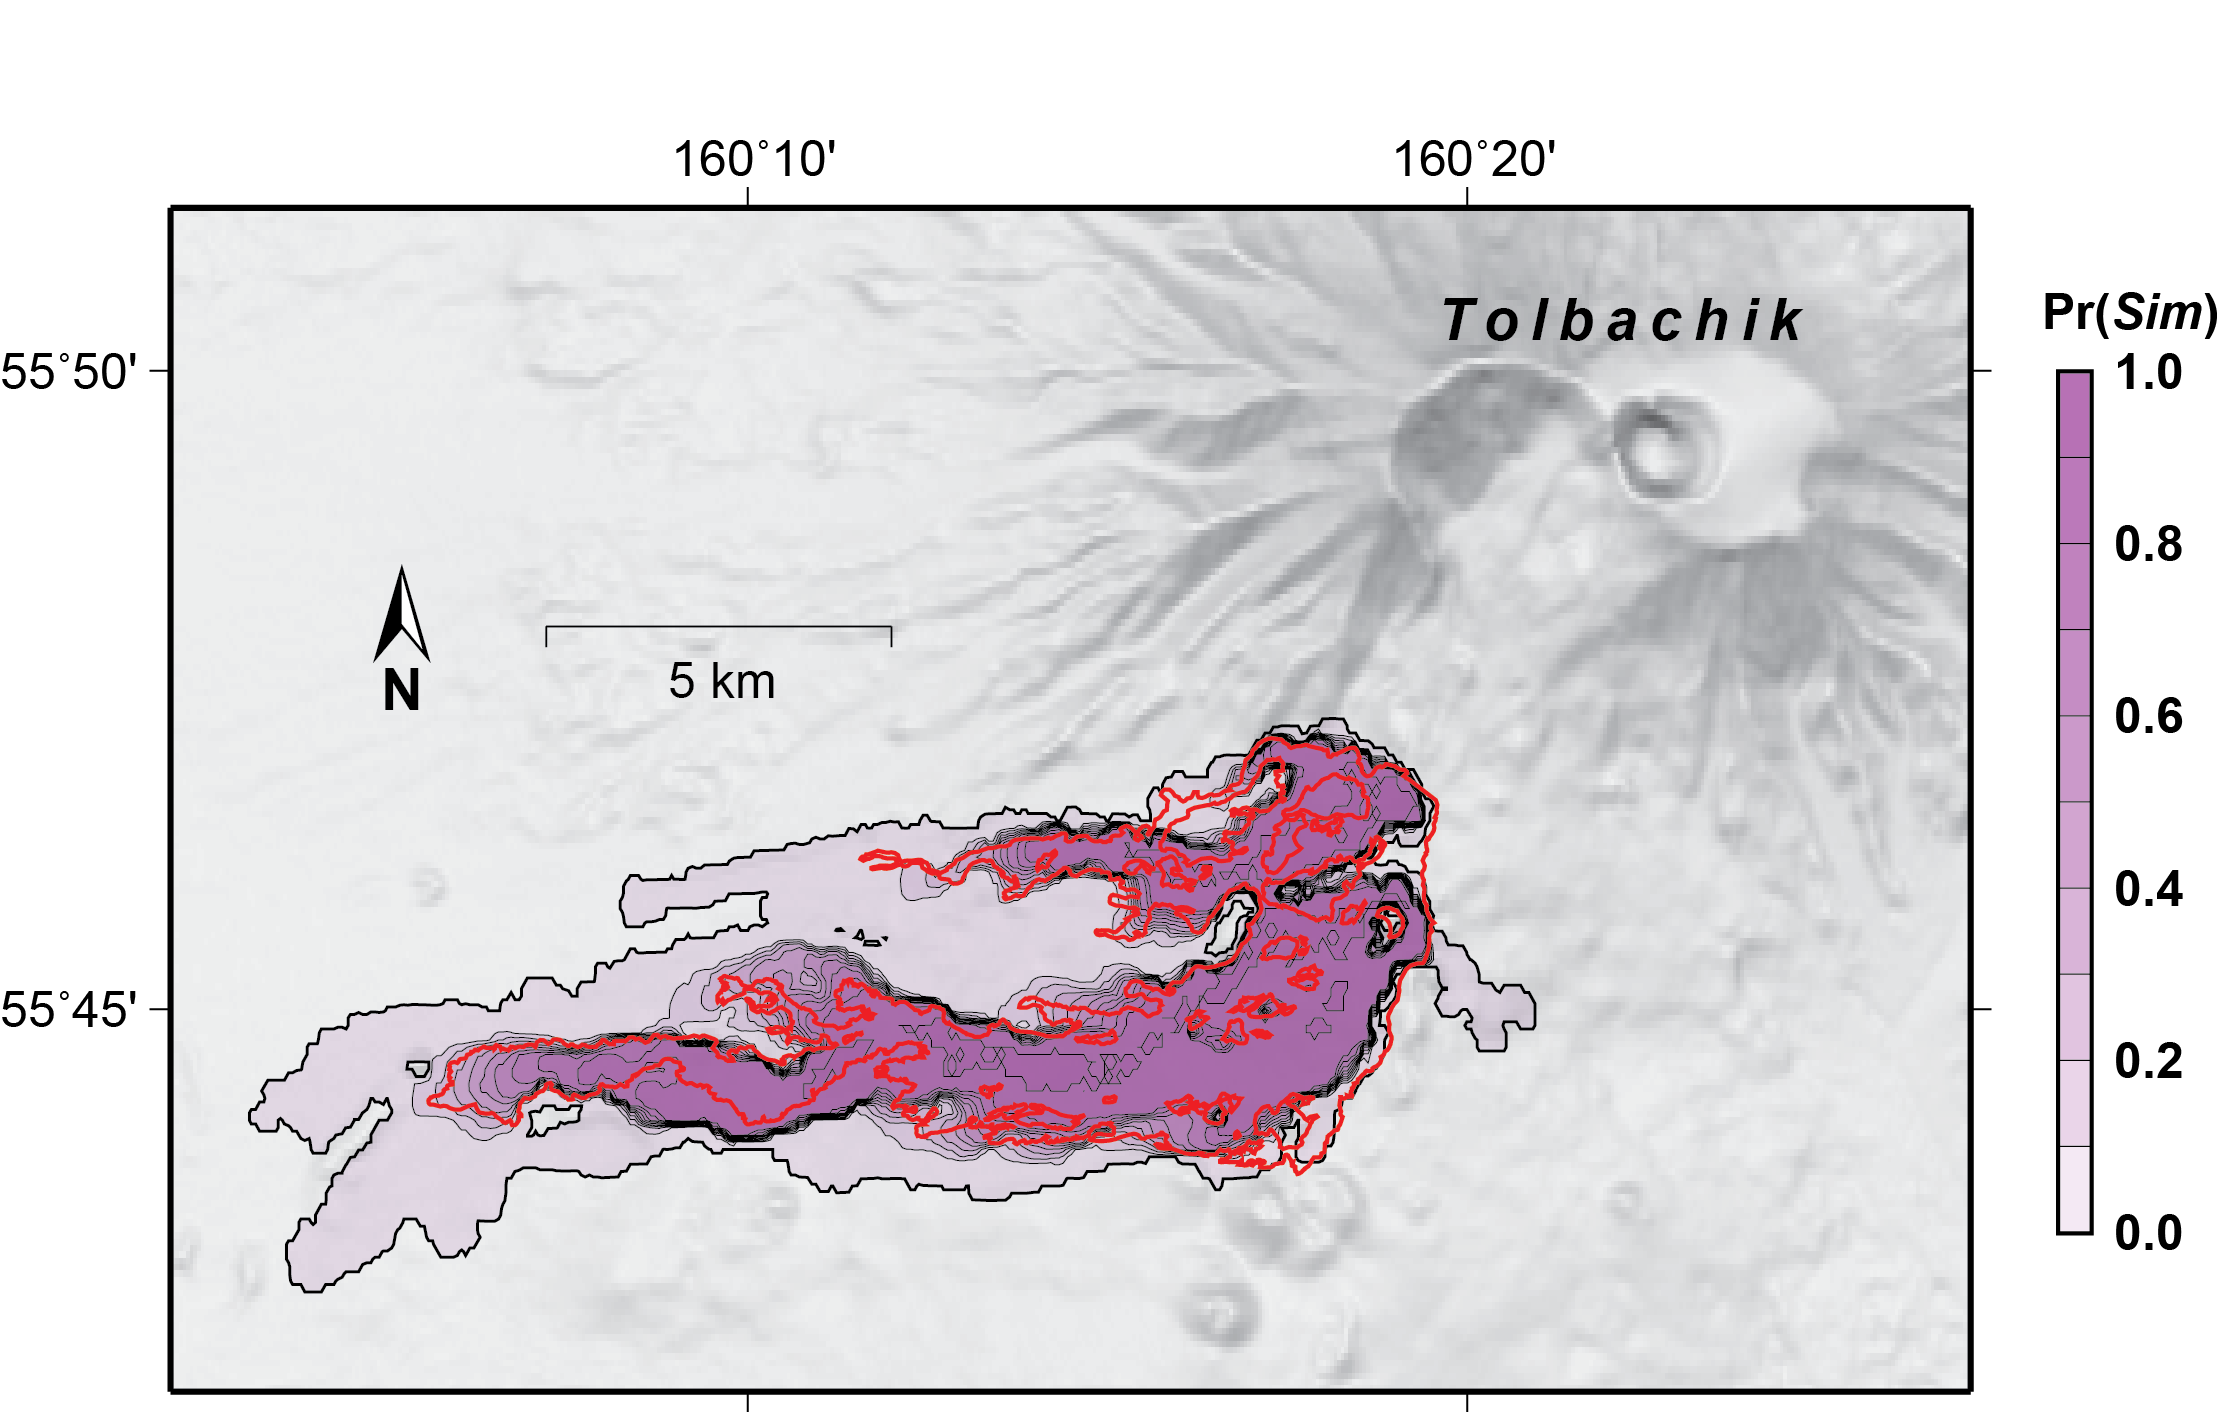
\includegraphics[width=0.7\linewidth]{\FigPath/MC_probmap_300dpi}
			\caption[Cumulative distribution of 100,000 simulated lava flows over SRTM topography with 3~m elevation uncertainty]{Cumulative distribution of 100,000 simulated lava flows over SRTM topography with 3~m elevation uncertainty. The red outline is the mapped flow extent of the 2012-3 Tolbachik flow. Darker purple areas represent more simulation hits (i.e. higher $\text{Pr}(Sim)$).}
			\label{fig_MC_map}
		\end{figure}
		
		The Monte Carlo method runs MOLASSES 100,000 times over a 75-m SRTM DEM. Vertical uncertainty of this data is estimated by \citet{rodriguez2006global} for Eurasia to be 6.2~m at a 90\% confidence level and is shown to be randomly distributed. With this result, elevation uncertainty in the MOLASSES model is given a value of $1\sigma=3$~m. Other input parameters remain unchanged from the validation exercise above; MOLASSES flow parameters for the Monte Carlo model are listed in Table \ref{tab_parameters_MC}. The combined 100,000 simulations are mapped in Figure \ref{fig_MC_map} where flow color indicates the number of flows that impacted each location.
		

				
		\subsubsection{Bayesian distribution of MC results}
			The reliability of a model can be better understood by showing the distribution of model performance given model uncertainty, as opposed to treating model parameters, and thus model output, as completely certain.  Figure \ref{fig:MC_dist} shows the distribution of PPV and NPV scores. Each dot in the main chart of Figure \ref{fig:MC_dist} represents a single flow simulation over a partially randomly generated DEM. The clustering of these points shows a positive correlation between the two predictive values, and both metrics are not normally distributed as shown on the histograms on either side of the main chart of Figure \ref{fig:MC_dist}. The flow simulation assuming no elevation uncertainty (shown in the top right corner of Figure \ref{fig:tolbachik}) fits the mapped flow better than the median value of both predictive values in the distribution, though it still lays within the MC distribution.
			
		%Graph of the performances
		\begin{figure}[h!]
			\centering
			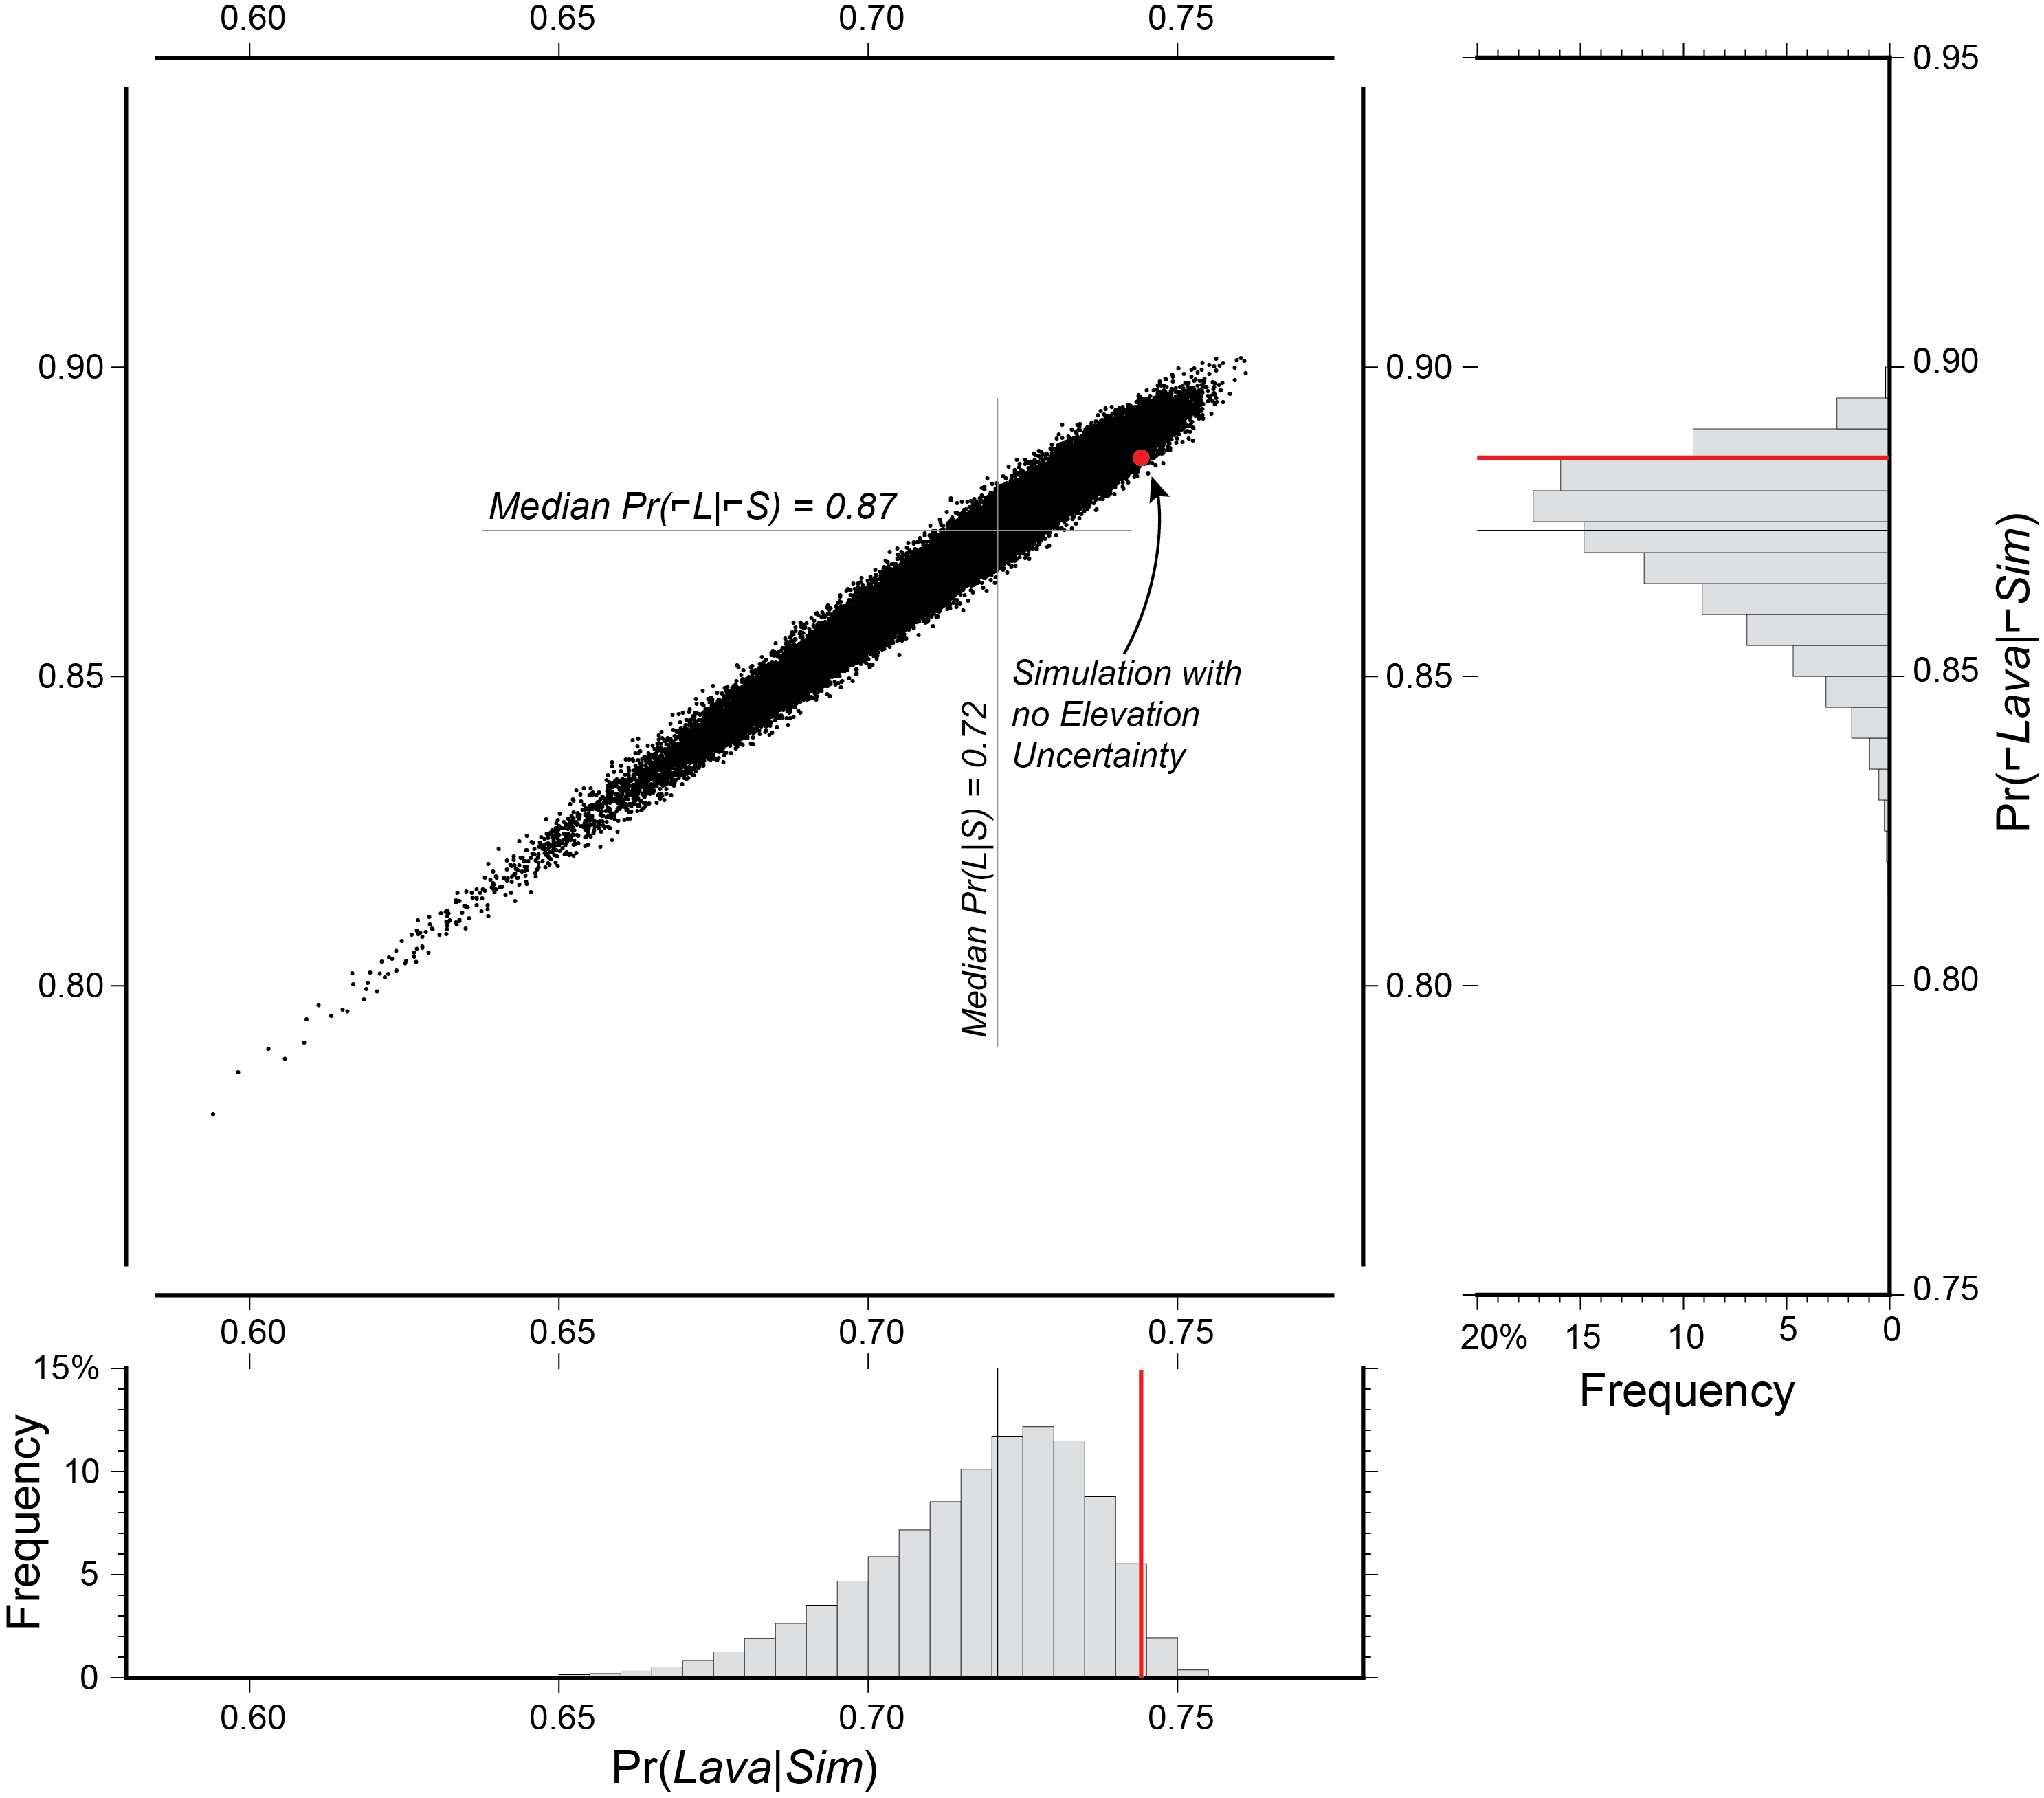
\includegraphics[width=0.7\linewidth]{\FigPath/MC_posteriors_300dpi}
			\caption[Fitness statistic distribution of Monte Carlo simulations of the 2012-3 Tolbachik lava flows, over SRTM topography with 3~m standard elevation uncertainty]{Fitness statistic distribution for 100,000 simulations of the 2012-3 Tolbachik Lava Flows, over SRTM topography with 3~m standard elevation uncertainty. Each point represents the predictive values of inundation/non-inundation for one simulation. Red lines are the fitness values of a simulated flow over SRTM data assuming 0~m elevation uncertainty (top right corner of Figure \ref{fig:tolbachik}). Black lines are placed at the median values of each predictive value.}
			\label{fig:MC_dist}
		\end{figure}
			
			If the elevation model used were perfect, the predictive values would be a single number ($\text{Pr}(Lava|Sim)=74.4$\% and $\text{Pr}(\neg Lava|\neg Sim)=88.5$\%). However, because elevation values have inherent uncertainty, model fitness, as defined by the predictive values, can be given as a range. Including elevation uncertainty, the $\text{Pr}(Lava|Sim)$ fitness has a range of 59-76\% and the $\text{Pr}(\neg Lava|\neg Sim)$ has a range of 77-91\%.


		\subsubsection{Estimating inundation risk from the simulated frequency of inundation}
		Figure \ref{fig_MC_map} shows a map view of the probability of inundation from the 100,000 MC simulations. Generally, areas within the mapped flow appear to be inundated by more simulations than outside the mapped flow. But can the probability of simulation inundation, $\text{Pr}(Sim)$, be used in a more formal way to judge the probability of lava inundation? In this section, the Tolbachik region map will be split into sub-regions based on $\text{Pr}(Sim)$, and the probabilities of inundation and not inundation will be compared.
		
		Three example sub-regions are shown in Figure \ref{fig_MCsubregions}. These sub-regions are defined as the area where $\text{Pr}(Sim)$ falls between a 10\% range. For instance, the top sub-region in Figure \ref{fig_MCsubregions} shows all locations that were forecast as inundated by at least 90\% of all MC simulations, while the middle sub-region example contains all locations inundated by 40-50\% of simulations. The sub-regions indundated by 0-10\% and 90-100\% of simulations are the largest sub-regions, while other sub-regions are thin rings between these two bounding sub-regions.
		
		\begin{figure}[!h]
			\centering
			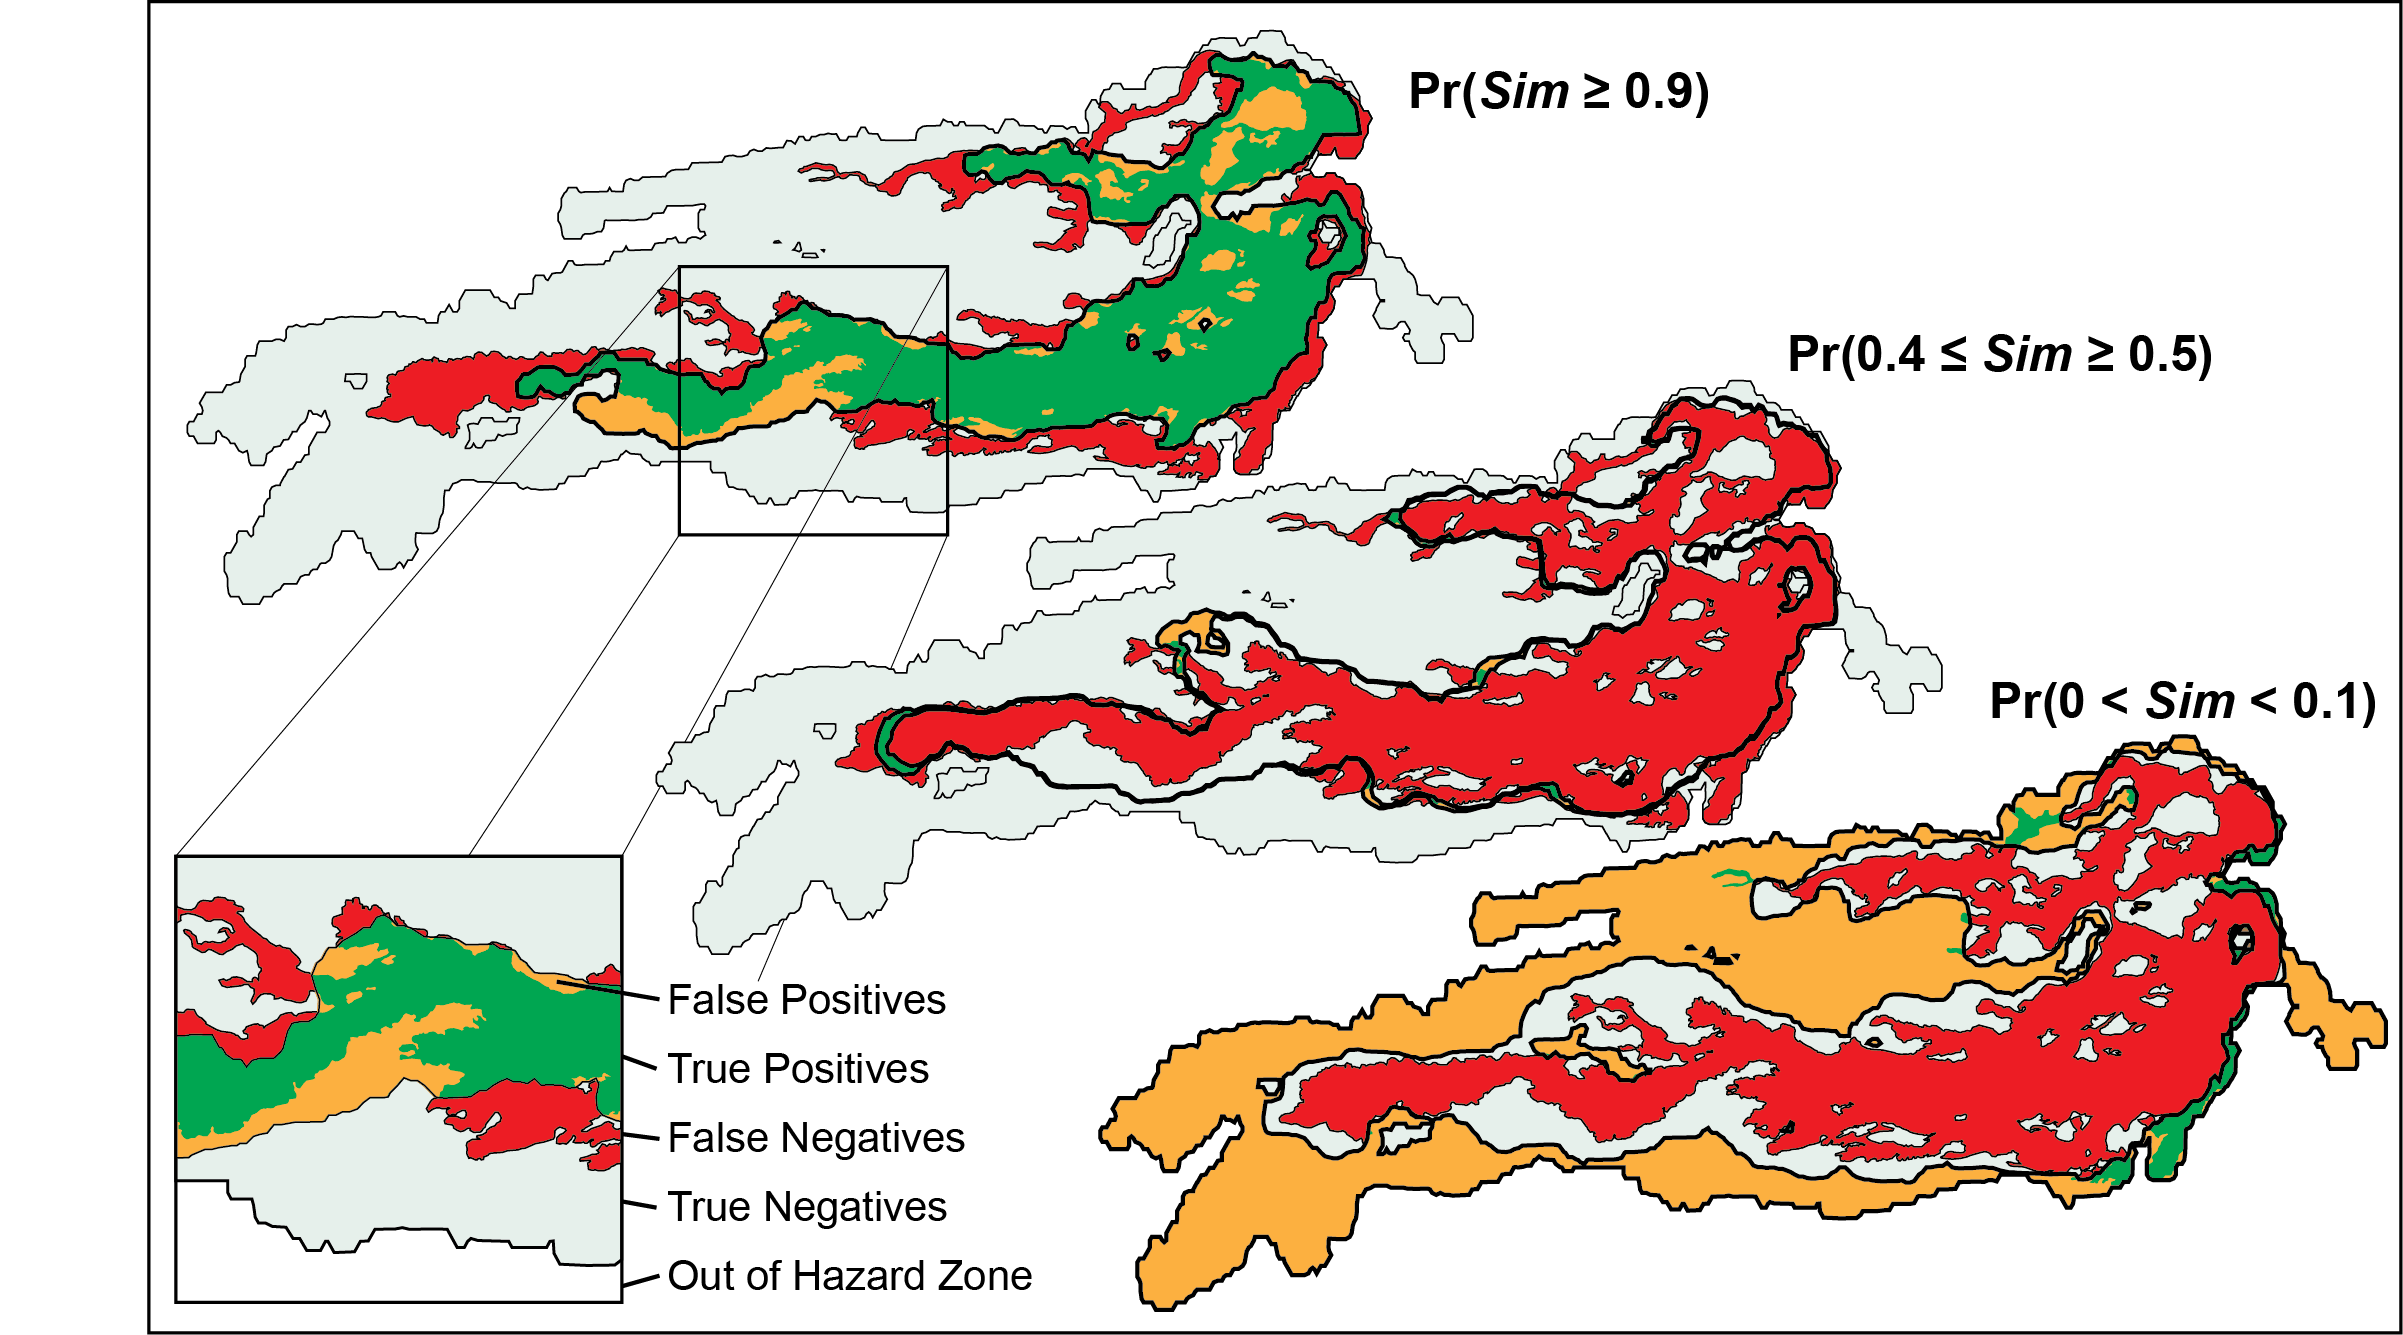
\includegraphics[width=0.7\linewidth]{\FigPath/PR_sim_examples_300dpi}
			\caption[Sub-regions within the Monte Carlo solution, defined by $\text{Pr}(Sim)$]{Sub-regions within the Monte Carlo solution, defined by $\text{Pr}(Sim)$. At the top, all areas inundated by $\ge$90\% of all simulations are shown in green (True Positives) and orange (False Positives). The remaining mapped lava flow (False Negatives) is red. The underlying region is the total Monte Carlo Hazard Area. At center, A thin band represents all areas inundated by 40-50\% of all Simulations. At bottom, a thick shell of areas rarely inundated by simulated lava is mostly orange, indicating rarely simulated flow areas are unlikely to have been inundated in real life.}
			\label{fig_MCsubregions}
		\end{figure}	
		
		It can be seen in Figure \ref{fig_MCsubregions} that most of the mapped flow is covered by the $\text{Pr}(Sim\ge90\%)$ sub-region, as the green true positive region is larger than the red false negative region. The sub-region defined as $\text{Pr}(0<Sim<10\%)$ does not spatially intersect with the mapped flow area as much as the $\text{Pr}(Sim\ge90\%)$ sub-region, and this can be seen in the lower right of Figure \ref{fig_MCsubregions} as the sub-region area is mostly orange false positives with small green true positive areas.
		
		The relative risk of inundation can be calculated for each subregion by comparing the probability of actual flow inundation $\text{Pr}(Lava)$ against the probability of not inundation $\text{Pr}(\neg Lava)$ using the Bayes Factor of Equation \ref{eq_BF}. Here the Evidence provided by the MC simulation is the probability of simulated inundation $\text{Pr}(Sim=\text{X})$ for a given area. Hypothesis 1 is that an area with a given probability of simulated inundation can be described as inundated by actual lava (``Inundation''). The opposing and complementary Hypothesis 2 is that this area can be described as not being inundated by actual lava (``Not Inundation''). For example, the relative probability of inundation for the sub-region defined by $\text{Pr}(40\le Sim<50\%)$ can be given as
		\begin{equation}
			\text{BF} = \frac{\text{Pr}(0.4\le Sim<0.5~|~\text{Inundation})}{\text{Pr}(0.4\le Sim<0.5~|~\text{Not~Inundation})}.
		\end{equation}
		The numerator $\text{Pr}(0.4\le Sim<0.5~|~\text{Inundation})$ is the probability of 40-50\% of simulations hitting a given location, given that location is actually engulfed by lava. Graphically, this is the percent of the true flow (red and green areas in the center example of Figure \ref{fig_MCsubregions}) that are within the simulated sub-region (True Positive green areas in the center example of Figure \ref{fig_MCsubregions}). The denominator $\text{Pr}(0.4\le Sim<0.5~|~\text{Not Inundation})$ is probability of 40-50\% of simulations hitting a location, given that location is not actually inundated by the real flow. This is the percent of the area not hit by the flow (light gray and orange areas in Figure \ref{fig_MCsubregions}) that is within the False Positives subregion (orange areas in Figure \ref{fig_MCsubregions}). 
		
		The probability that 40-50\% of simulations hit a location that is inundated is 2.7\%. The probability the 40-50\% of simulations hit a location that is not inundated by lava is 2.1\%. The Bayes Factor is then calculated to be 1.3, where the model of Inundation is 1.3 times more likely to describe this subregion than the model of Not Inundation. Referring to Table \ref{tab_BFinterps}, this result means that the preference for Inundation over Not Inundation is ``just worth a mention.'' Results for each 10\% wide sub-region are given in Table \ref{tab_BFresults} and are illustrated in Figure \ref{fig_bayesfactor}.
		

		\begin{table}
			\centering
			\caption{Relative likelihood of inundation given $\text{Pr}(Sim)$}
			\begin{tabular}{l c c c l}
				\toprule
				 & $\text{Pr}(Sim$=X$|$ & $\text{Pr}(Sim$=X$|$ & Bayes & \citet{jeffreys1998theory}\\
				X & $Lava)$ & $\neg Lava)$ & Factor & Interpretation \\
				\midrule
				$0<$X$<0.1$ & 0.06 & 0.67 & 0.09 & Strong evidence against inundation\\
				$0.1\le$X$<0.2$ & 0.02 & 0.08 & 0.23 & Substantial evidence against inund.\\
				$0.2\le$X$<0.3$ & 0.03 & 0.04 & 0.74 & No Inundation more likely\\
				$0.3\le$X$<0.4$ & 0.03 & 0.03 & 1.21 & Inundation more likely than not\\
				$0.4\le$X$<0.5$ & 0.03 & 0.02 & 1.29 & Inundation more likely than not\\
				$0.5\le$X$<0.6$ & 0.03 & 0.02 & 1.53 & Inundation more likely than not\\
				$0.6\le$X$<0.7$ & 0.04 & 0.01 & 2.63 & Inundation more likely than not\\
				$0.7\le$X$<0.8$ & 0.05 & 0.02 & 2.69 & Inundation more likely than not\\
				$0.8\le$X$<0.9$ & 0.06 & 0.02 & 2.84 & Inundation more likely than not\\
				$0.9\le$X$\le 1.0$ & 0.66 & 0.10 & 6.93 & Substantial evidence for inundation\\
				\bottomrule
			\end{tabular}
			\label{tab_BFresults}
		\end{table}
		
		\begin{figure}[!h]
			\centering
			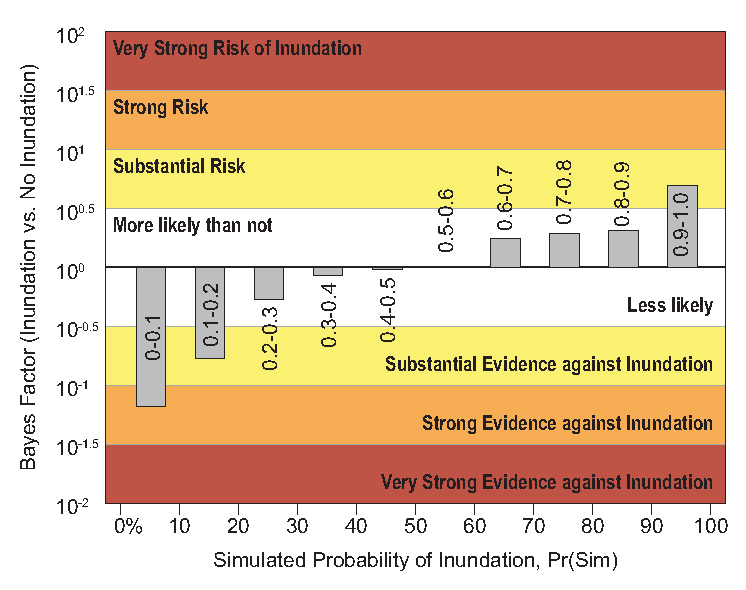
\includegraphics[width=0.7\linewidth]{\FigPath/LR_bayes}
			\caption[Relative likelihood of inundation given $\text{Pr}(Sim)$]{Relative likelihood of inundation given $\text{Pr}(Sim)$. Only locations inundated by $<10\%$ of Monte Carlo simulations show strong evidence against inundation in the actual 2012-3 Tolbachik lava flows.}
			\label{fig_bayesfactor}
		\end{figure}
		
		Only the sub-region least likely to be hit by simulations, where $\text{Pr}(Sim<10\%)$, has a Bayes Factor of $<10^{-1}$, which is interpreted as strong evidence against lava flow inundation. As the Bayes Factor can be treated as posterior odds for or against a model \citep{aspinall2003evidence}, a factor of $1/10$ indicates 10:1 odds against inundation. Sub-regions with factors greater than $1/10$, and are therefore more in support of flow inundation, have odds less than 10:1 against inundation. As 10:1 odds against inundation is the same as a probability of 9\% for inundation, all sub-regions besides the $\text{Pr}(Sim<10\%)$ sub-region have $\text{Pr}(Lava>9\%)$.
		


%%%%%%%%%%%%%%%%%%%%%%%%%%%%%%%%%%%%%%%%%%%%%%%%
%DISCUSSION
%%%%%%%%%%%%%%%%%%%%%%%%%%%%%%%%%%%%%%%%%%%%%%%%
%%%%%%%%%%%%%%%%%%%%%%%%%%%%%%%%%%%%%%%%%%%%%%%%
%%%%%%%%%%%%%%%%%%%%%%%%%%%%%%%%%%%%%%%%%%%%%%%%

\section{Discussion}\label{sec:discussion}
	\subsection{Validation of MOLASSES models}
	Unique flow algorithms are validated by using common tests that show whether these algorithms replicate expected lava flow morphologies under specific conditions. Different tests that are applicable to CA codes fall into three validation levels: 1) tests that show that simulations don't change when parameters remain meaningfully identical; 2) tests that show that simulations replicate experimental results or analytical expectations; and 3) tests that show that simulations replicate real world flow examples. A summary of the results of the eight algorithms against the example validation exercises are given below in Table \ref{tab_algorithmresults}.
		
	\begin{table}[h]
		\centering
		\caption{Transition Algorithm Results}
		\begin{tabular}{l | c | c | c c}
			\toprule
			Transition&\multicolumn{4}{c}{\textbf{Levels}}\\
			Function&1&2&\multicolumn{2}{c}{3}\\
			& DEM Rotation & Pancake & SRTM & TanDEM-X \\
			\midrule
			\textbf{4/P/S} & Pass & Fail & Pass & Pass\\
			\textbf{8/P/S} & Pass & Pass & Pass & Fail\\
			\textbf{4/N/S} & Fail & Fail & Pass & Fail\\
			\textbf{8/N/S} & Pass & Pass& Pass & Fail\\
			\textbf{4/P/E} & Fail & Ambiguous & Pass & Pass\\
			\textbf{8/P/E} & Fail & Ambiguous & Pass & Pass\\
			\textbf{4/N/E} & Fail & Pass & Pass & Pass\\
			\textbf{8/N/E} & Fail & Pass & Pass & Pass\\
			
			\bottomrule
		\end{tabular}
		\label{tab_algorithmresults}
	\end{table}
	
	Because these validation levels increase in complexity from Level 1 to Level 3, one possible strategy in validating different algorithms would be to only test algorithms at more complex levels after they successfully pass less complex tests. Valid models might then be determined by elimination. Only 3 of 8 tested algorithms pass the first ``rotating slope'' exercise: 4/P/S, 8/P/S, and 8/N/S. Although more algorithms passed the second ``bingham flow on a flat surface'' exercise, only 8/P/S and 8/N/S passed the previous exercise and this one. Both of these flows then successfully replicated the Tolbachik lava flows over SRTM topography. Therefore the 8/P/S and 8/N/S algorithms hold up to three tests.
	
	Overall, in all tests 8-connected models outperform 4-connected models. While equal sharing algorithms outperform slope-proportional sharing on a flat slope, they fail on a rotating DEM and perform about the same on real topography. There does not seem to be an unambiguously better choice between using parent-child relationships or not. If future tests continue to show similar performance between models with and without parentage, other reasons can be used to choose a model, such as computer run-time. 
	
	The strength of the MOLASSES code is that new algorithms, such as those used in the SCIARA model \citep{crisci2004simulation}, can be implemented relatively quickly and run through the validation exercises, which are written in Python. Combinations of implementation strategies can also be created on the fly by adjusting the makefile of the MOLASSES code instead of the code itself.

	\subsection{Bayesian applications for real lava flows}
		Validation of lava flow models is important as a method of increasing the value of models to forecast lava flow processes, thereby decreasing preventable loss. Flow models are generally improved by reducing false positives and false negatives while increasing the true positive area, which is the union of a flow simulation and real, mapped lava flows. Often, reducing one type of error comes at the cost of increasing another type. For example, by increasing the pulse volume parameter, false positives can be reduced while false negatives are increased (Figure \ref{fig:pulse_map}).
		
		A decision can be made as to whether false positives or false negatives are more important to reduce in calibrating a lava flow model. One possible decision would be to prefer the reduction of false negatives over the reduction of false positives, with the reason being that a forecast of inundation without eventual engulfment by lava (a false positive result) is bad, but an unexpected engulfment by lava (a false negative) would be worse.
		
		\subsubsection{Using Bayesian statistics to compare models}
		In Section \ref{sec_bayespulse}, an optimal pulse volume was defined as a volume that produced a simulated lava flow that had the highest PPV and NPV. However, the pulse volume 14040~m$^3$ had the highest PPV, while the pulse volume 4387~m$^3$ had the highest NPV. The simple definition of ``optimal'' pulse volume does not seem to work.
		
		The best pulse volume might be decided based on a preference for reducing false negatives as discussed above. The PPV of inundation, $\text{Pr}(Lava|Sim)$ increases with increased true positives and decreases with increased false positives (Equation \ref{eq_simplepost}). It is essentially blind to false negatives. The NPV $\text{Pr}(\neg Lava|\neg Sim)$ is the opposite, increasing with increased true negative results, while decreasing with increased false negative results (Equation \ref{eq_simplenegpost}). 
		
		If false negatives are more important to reduce than false positives, more weight can be given to the NPV of a simulation than the PPV. In Figure \ref{fig_weightedposteriors}, the PPV and NPV for each pulse volume (Figures \ref{fig_lavaGsim} and \ref{fig_neglavaGsim}) are used to produce weighted average scores of pulse volume. The extent to which false negative reduction might be preferred over false positive reduction is unknown, so four hypothetical weights are used. One of the weighted averages that is plotted assumes both predictive values are equally important in determining the best pulse volume parameter. The other three curves weigh NPV as being 2, 5, and 10 times as important as PPV in scoring pulse volumes. Using these three weights, the highest scoring pulse volume is 4387 m$^3$ (Figure \ref{fig:pulse_map}b). If the two values have equal importance, the highest scoring pulse volume is 14040 m$^3$ (Figure \ref{fig:pulse_map}c).
		
		\begin{figure}[h!]
			\centering
			\begin{gnuplot}[terminal=latex, terminaloptions=rotate]
				unset key
				set size 0.7,0.7
				set format xy "$%g$"
				set xlabel "Pulse Volume (m$^3$)" rotate by 90
				set ylabel "Model Score"
				set ytics 0.02
				set xtics 4000
				plot "data/results_bayes.dat" using 1:7 with points pt 1, "data/results_bayes.dat" using 1:5 with points pt 7, "data/results_bayes.dat" using 1:6 with points pt 3, "data/results_bayes.dat" using 1:4 with points pt 6
			\end{gnuplot}
			\caption[Weighted averages of $\text{Pr}(Lava|Sim)$ and $\text{Pr}(\neg Lava|\neg Sim)$ for different pulse volumes]{Weighted averages of $\text{Pr}(Lava|Sim)$ and $\text{Pr}(\neg Lava|\neg Sim)$ for different pulse volumes. Hollow circles, NPV ($\text{Pr}(Lava|Sim)$) is given 10$\times$ the weight of the PPV ($\text{Pr}(\neg Lava|\neg Sim)$); solid circles, 5$\times$ weight; asterisks, 2$\times$ weight; plusses, equal weight between predictive values. The highest scoring pulse volume is 4387 m$^3$ for all weight ratios except when both values are weighted equally.}
			\label{fig_weightedposteriors}
		\end{figure}
		
	\subsubsection{Decision making with the Bayes Factor}
	By dividing the Monte Carlo set of simulations of the Tolbachik lava flows into sub-regions based on $\text{Pr}(Sim)$, the relative likelihood of inundation was calculated (Figure \ref{fig_bayesfactor}). By using the Bayes Factor to compare likelihood of Indundation to Not Inundation, most sub-regions were not significantly better described by one model or the other. Only the sub-region of locations least likely to be hit by flow simulations had ``strong evidence'' against inundation, and only the sub-region of locations most likely to be hit by simulations had ``substantial risk'' of inundation. These results leave a large amount of ambiguity when making decisions to fortify or evacuate due to a lava flow.
	
	In discussing the decision making process for calling an evacuation due to an eruption at Mount Vesuvius, \citet{marzocchi2007probabilistic} provided a cost-loss model where two actions can be taken, protect and do not protect. Two costs are associated with these actions: $\mathcal{C}$ is the cost of protection and $\mathcal{L}$ is the cost of loss if the volcanic hazard occurs while a decision to not protect is made. If $\mathcal{L}$ is incurred, it is assumed to exceed cost $\mathcal{C}$, often because loss due to volcanic hazards includes the loss of life.
	
	\citet{marzocchi2007probabilistic} show that the minimum cost can be achieved if protection occurs when $p>\mathcal{C}/\mathcal{L}$ where $p$ is the probability of the hazard occuring. The ratio $\mathcal{C}/\mathcal{L}$ is hard to quantify because the socio-economic cost of lost lives or of lost trust in the government (in the case of false evacuations) is difficult to calculate, even though the physical cost of evacuation and the cost of infrastructure loss might be straight forward estimates. \citet{woo2008probabilistic} provided one estimate of $\mathcal{C}/\mathcal{L}=0.1$ at the very maximum if 10\% of people evacuated from an area would owe their lives to that evacuation. In this case, protection would be made when $p>0.1$.
	
	While lives are not commonly lost due to lava flows with the notable exceptions of Laki (A.D. 1783, Iceland) and Nyiragongo (A.D. 1977 and 2002, Democratic Republic of the Congo) \citep{peterson2000lava}, the ``protection threshold'' $p>0.1$ can still be used as an example. All Monte Carlo sub-regions have a probability of inundation ($\text{Pr}(Lava)$) greater than 0.1 except the sub-region $\text{Pr}(Sim<0.1)$ (Figure \ref{fig_bayesfactor}). If action to protect is made at $\text{Pr}(Lava>0.1)$, then evacuations or fortifications will be made for all locations inundated by $\ge$10\% of Monte Carlo simulations.
	
	Two Bayes-factor thresholds in Figure \ref{fig_bayesfactor} have odds against lava inundation at better than 10:1 (i.e. $\text{Pr}(Lava<0.1)$), ``strong evidence'' and ``very strong evidence'' against inundation. Given the hypothetical protection threshold of $p>0.1$, the decision to protect against a lava flow should be made for a location whenever the Bayes factor supporting inundation is $>10^{-1}$, or when there is less than ``strong evidence'' against inundation for that area. If the protection threshold is decided to be less than 0.1, then the evidence against inundation will have to be even stronger to support a decision to not protect an area. 
	
	It is unknown whether sub-regions defined as $\text{Pr}(Sim<0.1)$ should be expected to be relatively safe areas when using Monte Carlo results at future lava flow sites. To test the effectiveness of the MOLASSES algorithm used for the Tolbachik flows in other study areas, more example flows around the world will have to be tested.
		
		
\section{Conclusions}
	The MOLASSES framework used in this project provides a modular set of functions that can be interchanged to fundamentally alter the flow simulation algorithm. While only 8 different algorithms, which focused on simple variations in the transition function of Cellular Automata codes, were explored, different modules can feasibly be modified to change other flow characteristics (e.g. vent geometry, mass flux at source locations, temperature dependent flow).
	
	All CA and CA-like codes, including SCIARA \citep{crisci2004simulation}, MAGFLOW \citep{del2008simulations}, ELFM \citep{damiani2006lava}, LavaPL \citep{connor2012probabilistic}, and MOLASSES share similarities. For instance, lava inundation is a binary condition for each location on a grid and source locations are set at defined grid cell coordinates. This enables a common set of validation exercises to be defined, which can be used to test the validity of all CA codes.
	
	Three validation levels have been identified and different tests have been given which apply to each level. After a code is successfully demonstrated to conserve mass, the first validation level ensures that the code does not change when parameters are changed in a meaningless way. The example exercise is that simulated flows should not be slope-direction dependent. The second level compares simulations to analytical or experimental results. As lava flows on large scales are similar to Bingham fluids, a flow simulator should produce a circular pattern on a flat surface. The third and final level tests simulations against true lava flows. Here, the 2012-3 Tolbachik lava flow is used as an example, with flow parameters identified using TanDEM-X analysis \citep{kubanek2015lava}. It might only make sense to validate codes at higher validation levels once they have been sufficiently developed to be validated at lower levels.
	
	Two common fitness tests for lava flows are the Jaccard coefficient and model sensitivity. Model sensitivity gives the percentage of a mapped lava flow that a simulation successfully forecasts. A possible alternative to these tests is to use Bayesian posterior probabilities, or predictive values to evaluate the positive and negative predictive values of the simulation. These predictive values (PPV, $\text{Pr}(Lava|Sim)$; and NPV, $\text{Pr}(\neg Lava|\neg Sim)$) give the likelihood of flow inundation or not inundation given the simulation results.
	
	Once lava simulators have been successfully validated, these Bayesian statistics can be used to improve model input parameters and evaluate model uncertainty by incorporating uncertainty inherent in input parameters. It is also possible that the two predictive values can be used to aid in decision making processes associated with active lava flow crises.
	
	
\section{Data statement}
This code is available for free use on GitHub at the USFVolcanology page located at \url{https://github.com/USFvolcanology}, while the validation codes can be found at \url{https://github.com/jarichardson/MOLASSES_benchmarking}. The MOLASSES code and the validation algorithms are kept in seperate self-contained repositories.

\section{Notation}
	\begin{table}[h!]
		\centering
		\caption{Notation}
		\begin{tabular}{l l}
			\toprule
			\textbf{A}& Cellular Automata (CA) structure\\
			E$^2$& set of CA point locations\\
			V & set of source locations in E$^2$\\
			X & local neighborhood for each cell\\
			$n$ & an element of X\\
			S & set of subsets for each cell\\
			$\sigma$ & transition function of the CA\\
			$\gamma$ & source function of the CA\\
			$i$,$j$ & row, column location within E$^2$\\
			$c$ & the location of a central cell of interest\\
			$t$ & timestep in the CA\\
			S$_e$, S$_h$, S$_h0$ & elevation, lava thickness, and critical thickness of a cell\\
			V$_{in}$ & total volume delivered to source locations\\
			V$_{out}$ & total volume in all inundated cells\\
			$A_{flow}$ & total footprint area of a flow simulation\\
			$d_{max}$ & maximum distance of lava from the source location\\
			$N$ & the predefined hazard area\\
			$R_{max}$ & maximum hazard radius\\
			$\rho$ & density of lava flow crust\\
			$\epsilon$ & emprical extension-before-failure value\\
			$S$ & tensile crust strength\\
			$Q$ & mean volumetric flux\\
			$g$ & acceleration due to gravity\\
			$\kappa$ & bulk thermal diffusivity\\
			$\mathcal{C}$ & the cost of protection\\
			$\mathcal{L}$ & the cost of loss if protection does not occur\\
			$p$ & probability of hazard occuring\\
			\bottomrule
		\end{tabular}
		\label{tab_notation}
	\end{table}

%\section{Acknowledgments}
%The development of this code was supported by SSI Grant

%%%%%%%%%%%%%%%%%%%%%
%%References Section
%\section{References}

%\nobibliography{dissertation_refs}
%\bibliographystyle{apalike} 

%\begin{figure}
%\centering
%\includegraphics[width=\linewidth]{map_diff}
%\label{fig:map_diff}
%\end{figure}

